This example is presented to introduce \textit{bioptim}'s ability to deal with a multiphase locomotion estimation problem with muscle actuation and contact forces.
The goal was to estimate muscles activation by tracking markers trajectories and ground reaction forces and moments. 
The model was a 3D leg with 12 DoFs (6-DoFs pelvis + 3-DoFs hip + 1-DoF knee + 2-DoFs ankle), driven by 17 muscle activations and residual joint torques to compensate for potential actuation weaknesses. 
The gait cycle was defined from the first heel strike to the end of the swing phase discretized into shooting 90 intervals. 
To follow the natural rolling of the foot, the stance was divided into three phases (heel, flatfoot and forefoot contacts) of fixed duration deduced from experimental force platform data and markers position ($0.05$, $0.36$ and $0.16$s).
The swing phase lasted 0.38 s. 
The interaction between the ground and the foot was modeled using a 4-contact points model located at the heel and the forefoot (first, fifth metatarsi and hallux).
The optimization problem consisted in minimizing the errors between predicted $\bm{\mathcal{M}}$ and reference $\bm{\mathcal{M}}^*$ markers trajectories, predicted $\bf{f}$, $\bf{m}$ and reference $\bf{f^*}$, $\bf{m^*}$, respectively ground reaction forces and moments at all contact points.
A regularization term on muscle activations, $\bf{a}$, was also added (least-activations) as well as a penalization term on the residual torques $\boldsymbol{\tau}$:

\[ 
\resizebox{0.9\columnwidth}{!}{$ 
\begin{aligned}
%\mathcal{J} = &\int_{t=0}^{T}\underbrace{\omega_1(\|m_p - m_m\|^{2})}_{\mathtt{TRACK\_MARKERS}}~ 
%+ ~ \underbrace{\omega_2(\|f_p - f_c\|^{2})}_{\mathtt{TRACK\_FORCES}}\\
%&+ ~ \underbrace{\omega_3(\|tau^f_p - tau^f_m\|^{2})}_{\mathtt{TRACK\_MOMENTS}}~
\mathcal{J} = &\int_{t=0}^{T}\underbrace{\omega_1(\|\bm{\mathcal{M}} - \bm{\mathcal{M}}^*\|^{2})}_{\mathtt{TRACK\_MARKERS}}~ 
+ ~ \underbrace{\omega_2(\|\bf{f} - \bf{f}^*\|^{2})}_{\mathtt{TRACK\_FORCES}}\\
&+ ~ \underbrace{\omega_3(\|\bf{m} - \bf{m}^*\|^{2})}_{\mathtt{TRACK\_MOMENTS}}~
+ ~ \underbrace{\omega_4\|\bf{a}\|^2}_{\mathtt{MIN\_ACTIVATION}}
+ ~ \underbrace{\|\boldsymbol{\tau}\|^2}_{\mathtt{MIN\_TORQUE}}~dt, 
\end{aligned}  
$}  
\addtag  
\label{eq:ocp_walk}  
\]

\noindent where $\omega_1$=1e5, $\omega_2$=0.1, $\omega_3$=0.1, $\omega_4$=10 are  weighting factors and $T$ is the the duration, $N_i$ and $N_c$ are the number of time frames and contact points of the current phase. $^*$ stands for reference (i.e., measured) data.\\

Non-slipping ($\mathtt{NON\_SLIPPING}$) and unilateral contact force ($\mathtt{CONTACT\_FORCE}$) constraints prevented the foot from slipping and pulling from the ground. 
In between phases, the use of the $\mathtt{IMPACT}$ state transition allowed to represent the gain or loss of contact(s) in the dynamics (e.g., swing phase to heel strike [thesis Felis - articles?]) \\

Fig.~\ref{fig:snapshots_multiphase_walking_cycle} shows the leg motion during the walking cycle. 
The root mean square tracking error on markers trajectories was 0.027 m (mean error on pelvic and foot markers was 0.0075 m and 0.0147 m, respectively). 
Concerning ground reaction forces tracking, the root mean square error was 4.85 N.
Fig.~\ref{fig:muscles_activation_gait} shows muscle activity patterns during the gait cycle.
Gluteal muscles were only activated during the stance phase. The Gluteus Maximus was mainly activated during the early flatfoot phase with a maximal activation of 0.2 allowing to prepare the stance phase. 
For the thigh muscles, the semimembranous, semitendinous and biceps femoris were activated during the early stance phase and terminal swing (maximal activation of 0.3, 0.4 and 0.4, respectively) which is coherent with the activity patterns recorded from Winter (1991) [Winter DA (1991). The Biomechanics and Motor Control of Human Gait: Normal, Elderly and Pathological.].  
The knee extensors, vastus lateralis, medialis and intermedius followed the same pattern and were mainly activated during the flatfoot phase (ie loading response). Chang et al. (2007) observed a significant pre-swing and initial swing activity for those muscles which was found a bit earlier in this simulatiom (terminal stance).
However, while they observed highest activity of the rectus femoris at late swing and loading response (early flatfoot phase), the maximal activation appeared at  forefoot phase (terminal stance) and pre swing. [Chang et al (2007). https://doi.org/10.1016/j.jelekin.2006.02.003]["Five basic muscle activation patterns account for muscle activity during human locomotion" Ivanko et al. (2004)] 
Leg muscles were highly activated (saturation of gastocnemius lateralis and medialis) at the terminal stance and early swing. The tibialis anterior is the sole muscle for dorsiflexion and the only antagonist of the triceps surae in this model which could explain its high activity at the same time. 

\begin{figure*}[t!]
\centering
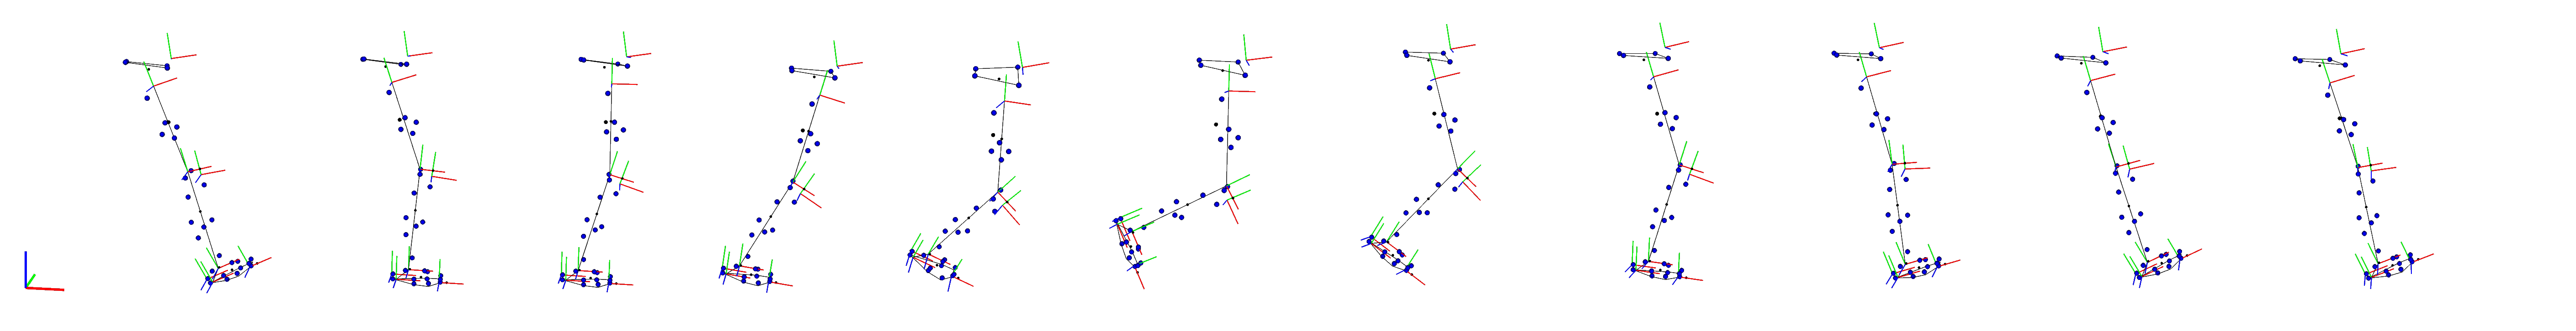
\includegraphics[width=\textwidth]{figures/multiphase_walking_cycle.png}\\
\caption{Snapshots of a walking gait cycle driven by muscles activation.}
\label{fig:snapshots_multiphase_walking_cycle}
\end{figure*}

\begin{figure*}[t!]
\centering
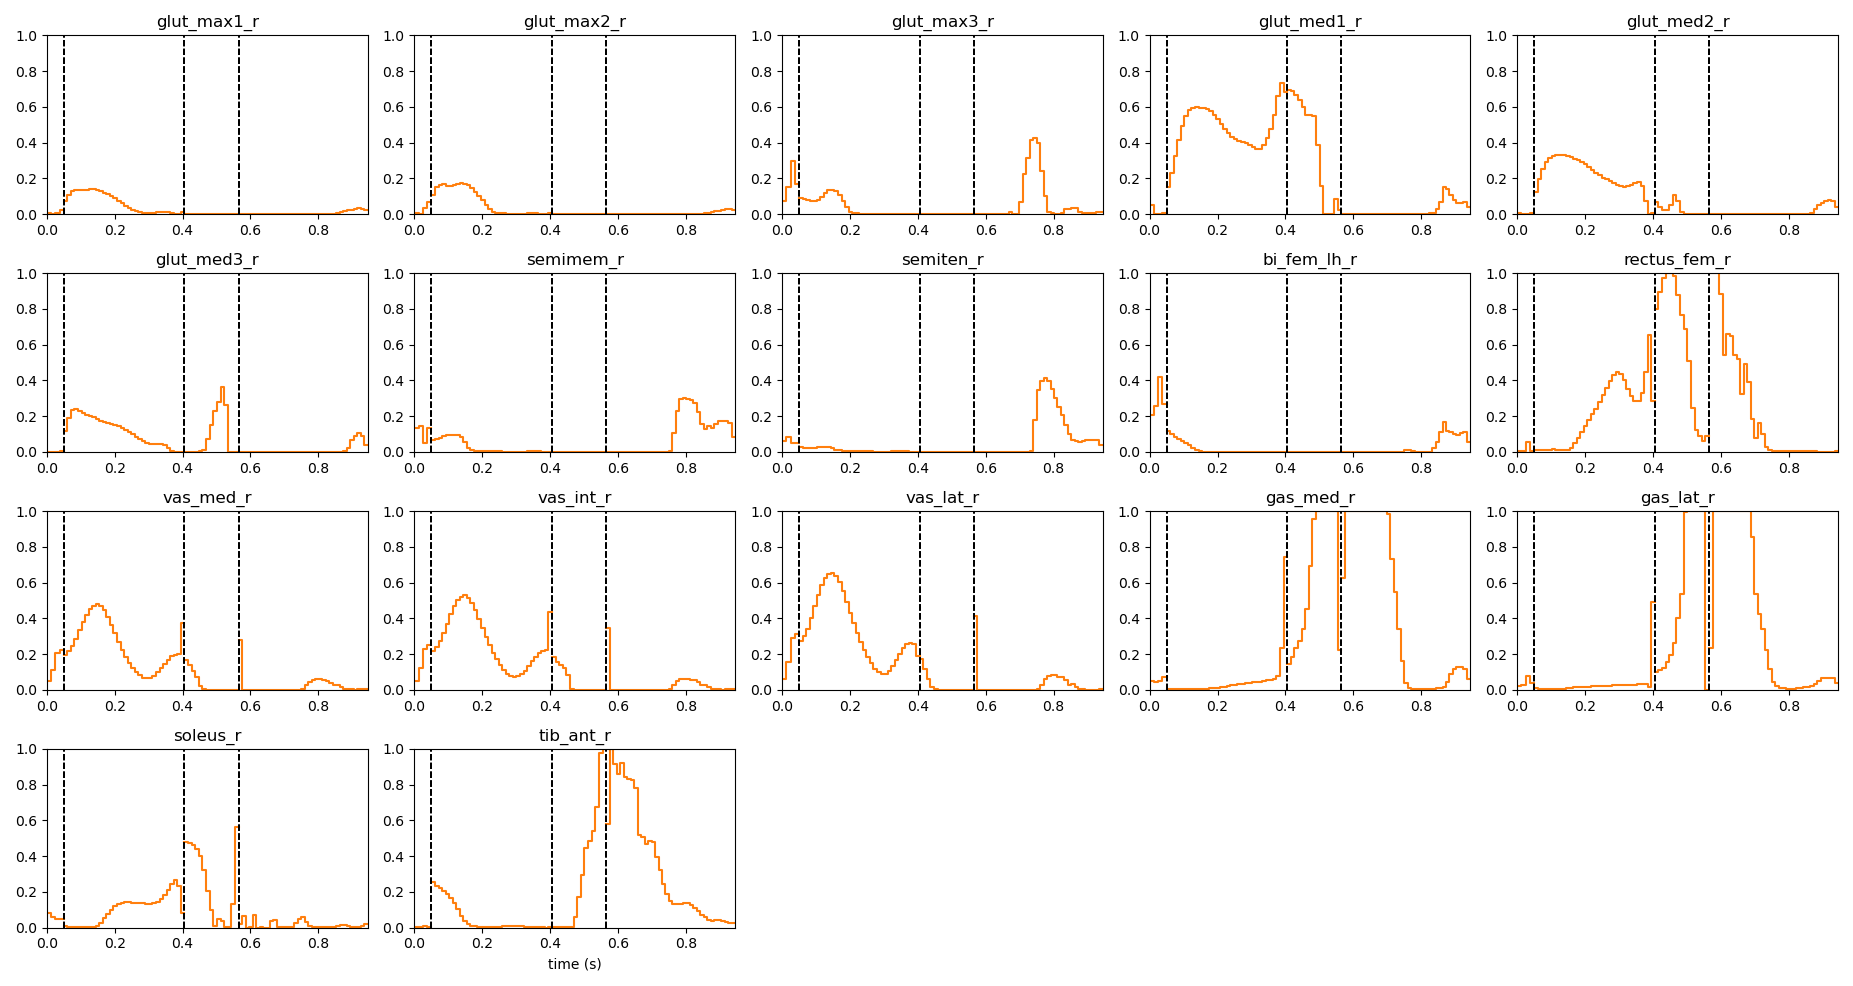
\includegraphics[width=\textwidth]{figures/muscles_control_gait_example.png}\\
\caption{Muscle activity patterns during walking cycle.}
\label{fig:muscles_activation_gait}
\end{figure*}
